\chapter{Activity Protocols}

\section{Debugging Activity}
The debugging activity embedded assessment was scaffolded by a short lecture presented by the researcher. The following pages include the slides from that lecture, followed by a description of the starter app provided to the students, and then the student worksheet.
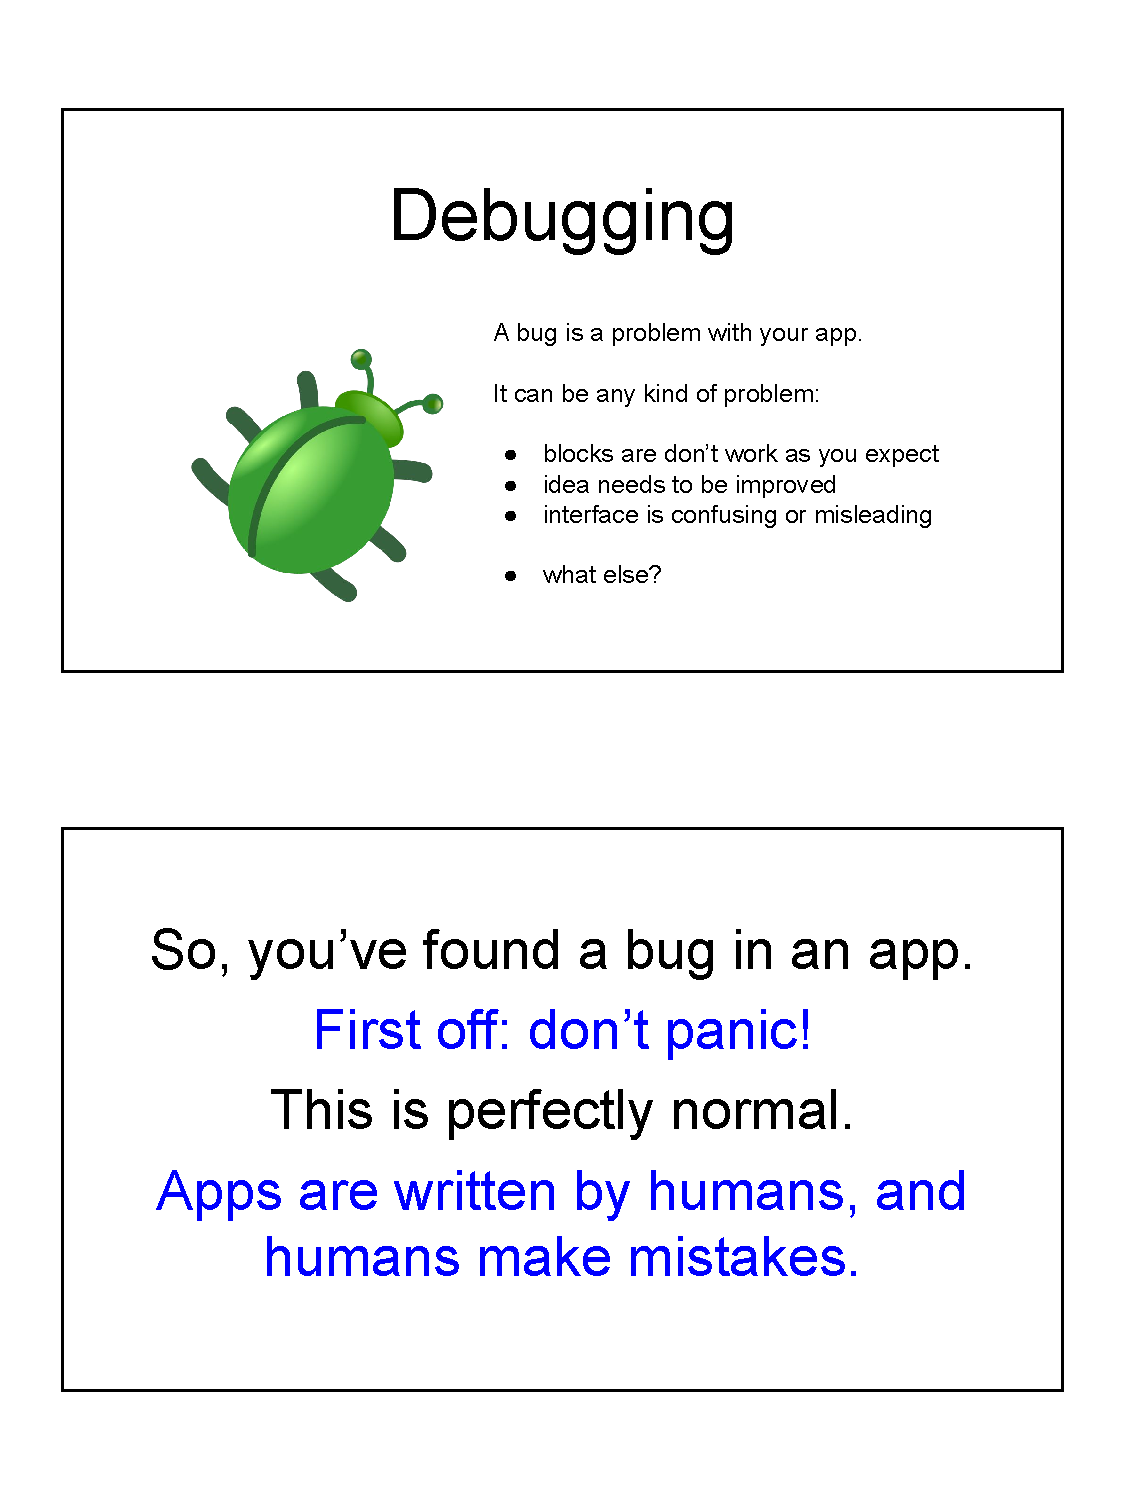
\includepdf[pages=-, frame, scale=.8]{IRB/Mark_Debugging_Lecture_handout.pdf}
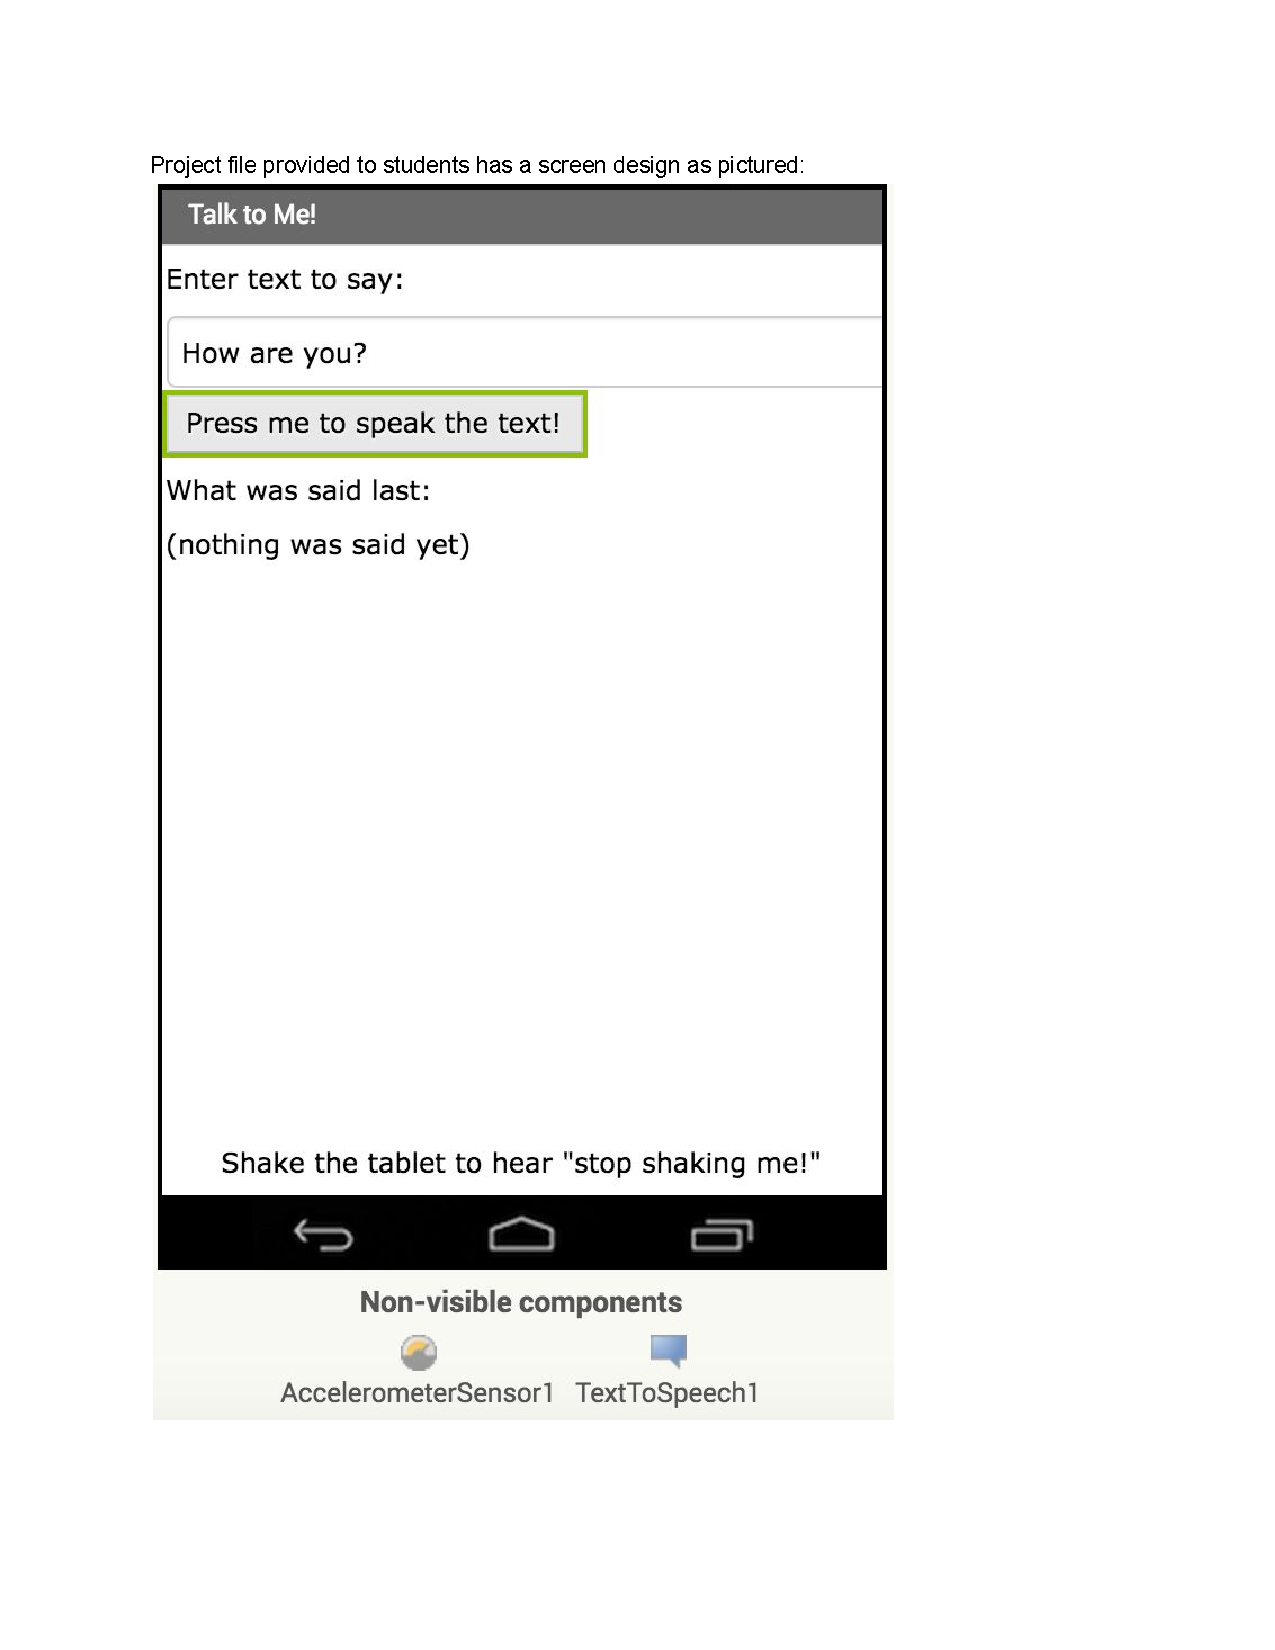
\includepdf[pages=-, frame, scale=.8]{IRB/AM10DebuggingAssessment.pdf}
\label{apx:debugging-protocol}

\section{Temperature Activity}
The temperature activity embedded assessment was conducted during the summer camp. The following pages include a description of the starter app and the student worksheet. This activity did not have a slide deck to accompany its scaffolding lecture, and one needs to be added for future implementations.
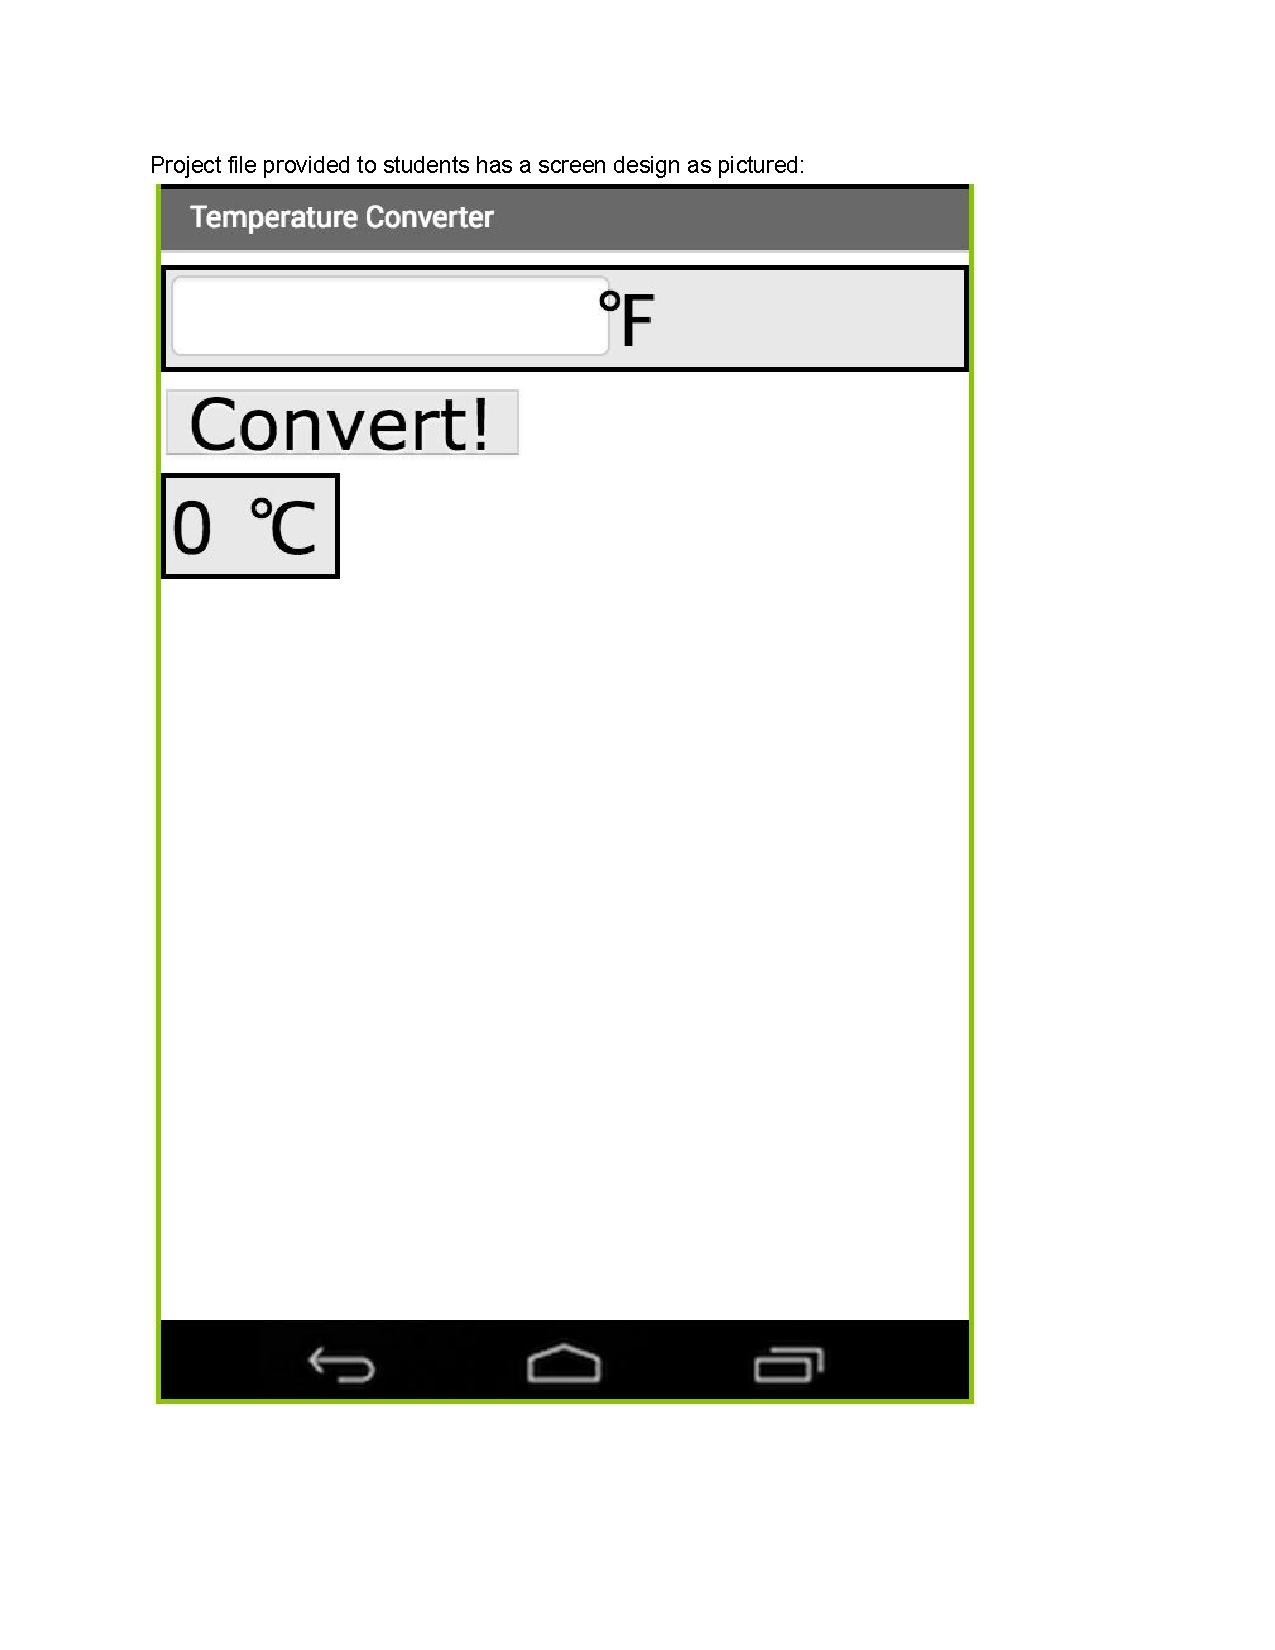
\includepdf[pages=-, frame, scale=.8]{IRB/AM10TemperatureAssessment.pdf}
\label{apx:temperature-protocol}

\chapter{Institutional Compliance Forms}
This project was monitored by the UMass Lowell Office of Institutional Compliance Institutional Review Board (IRB). This section contains the relevant submissions and approval letters between the research team and the IRB.

% \section{IRB Application}
% \label{IRB:app}
% "Middle School Pathways in Computer Science" was originally submitted by Fred Martin on June 25, 2014. Approval was received after expedited review on July 7, 2014, as IRB Protocol \# 14-144-MAR-XPD. The approval period was for July 7, 2014 through July 6, 2015.

% The following pages contain a copy of the IRB application form and the approval letter in response.

% 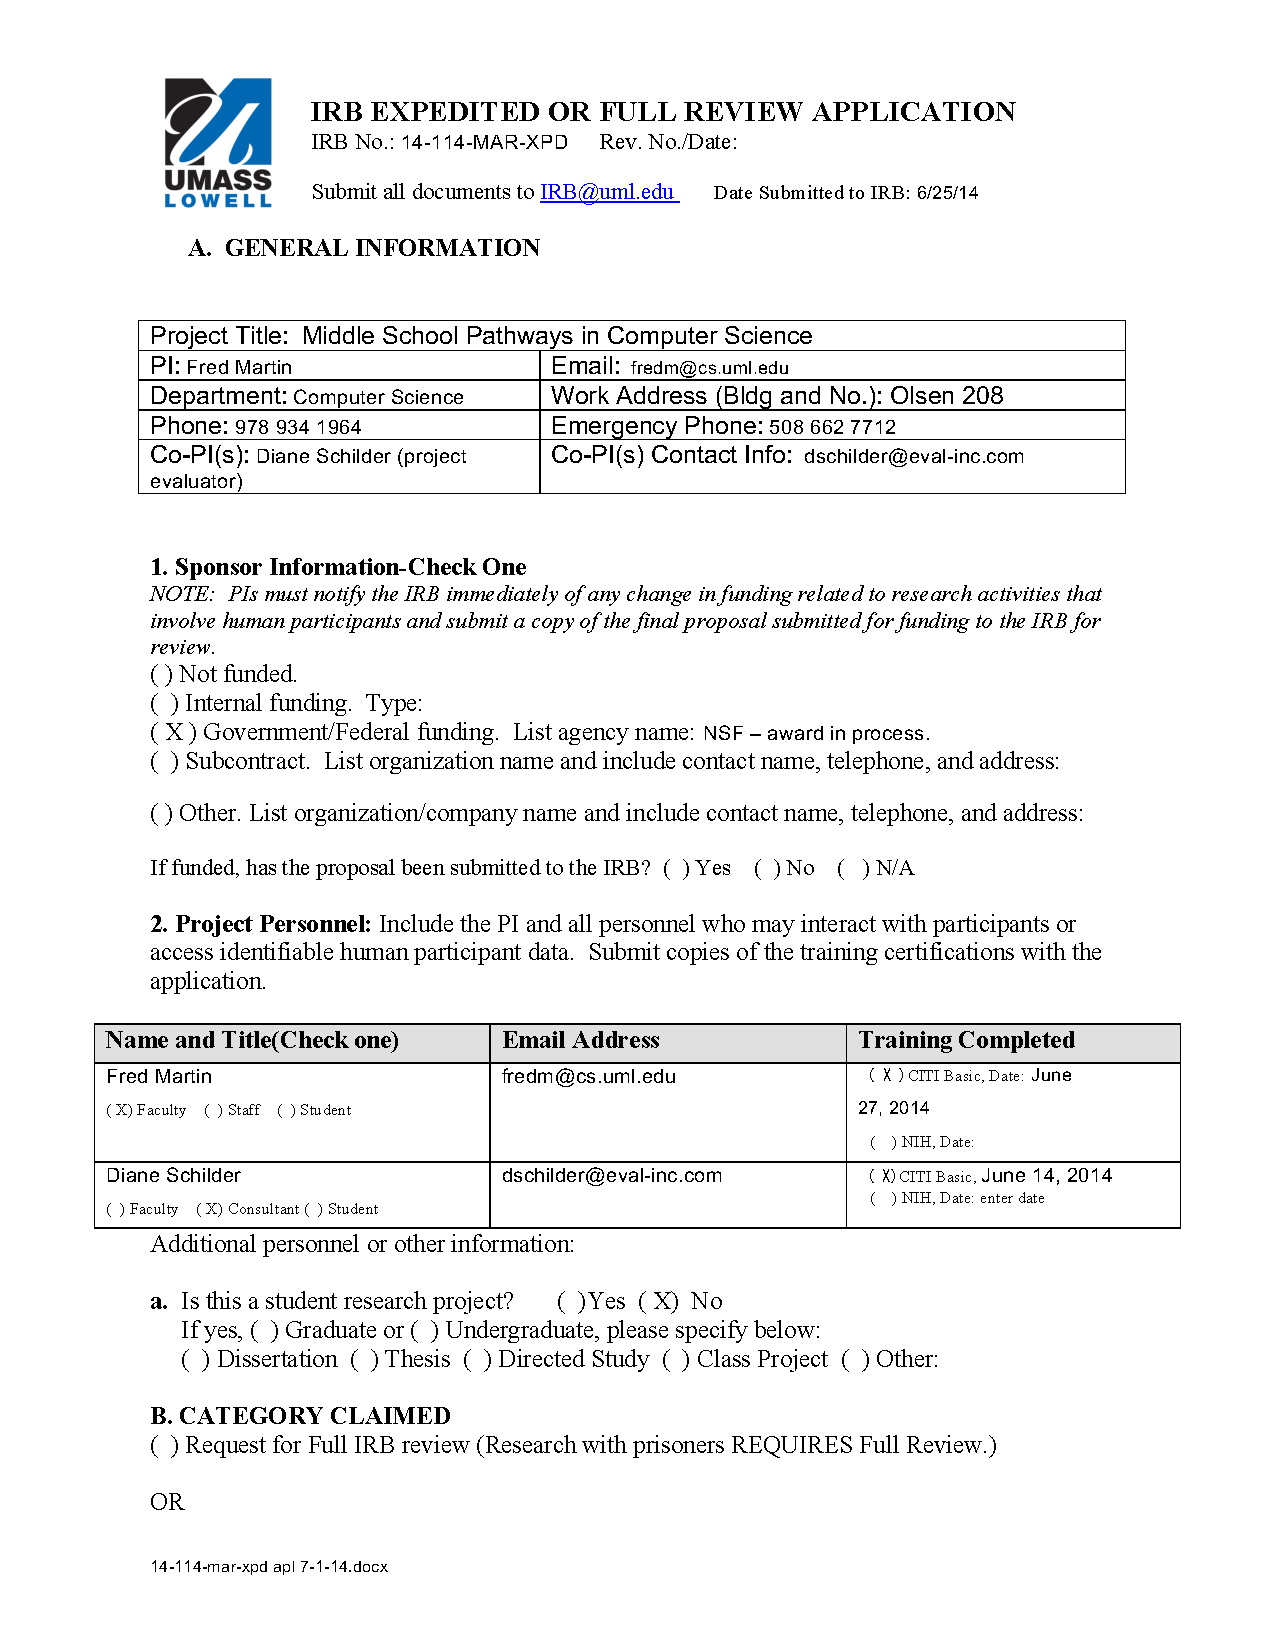
\includepdf[pages=-]{IRB/14-144-app.pdf}
% 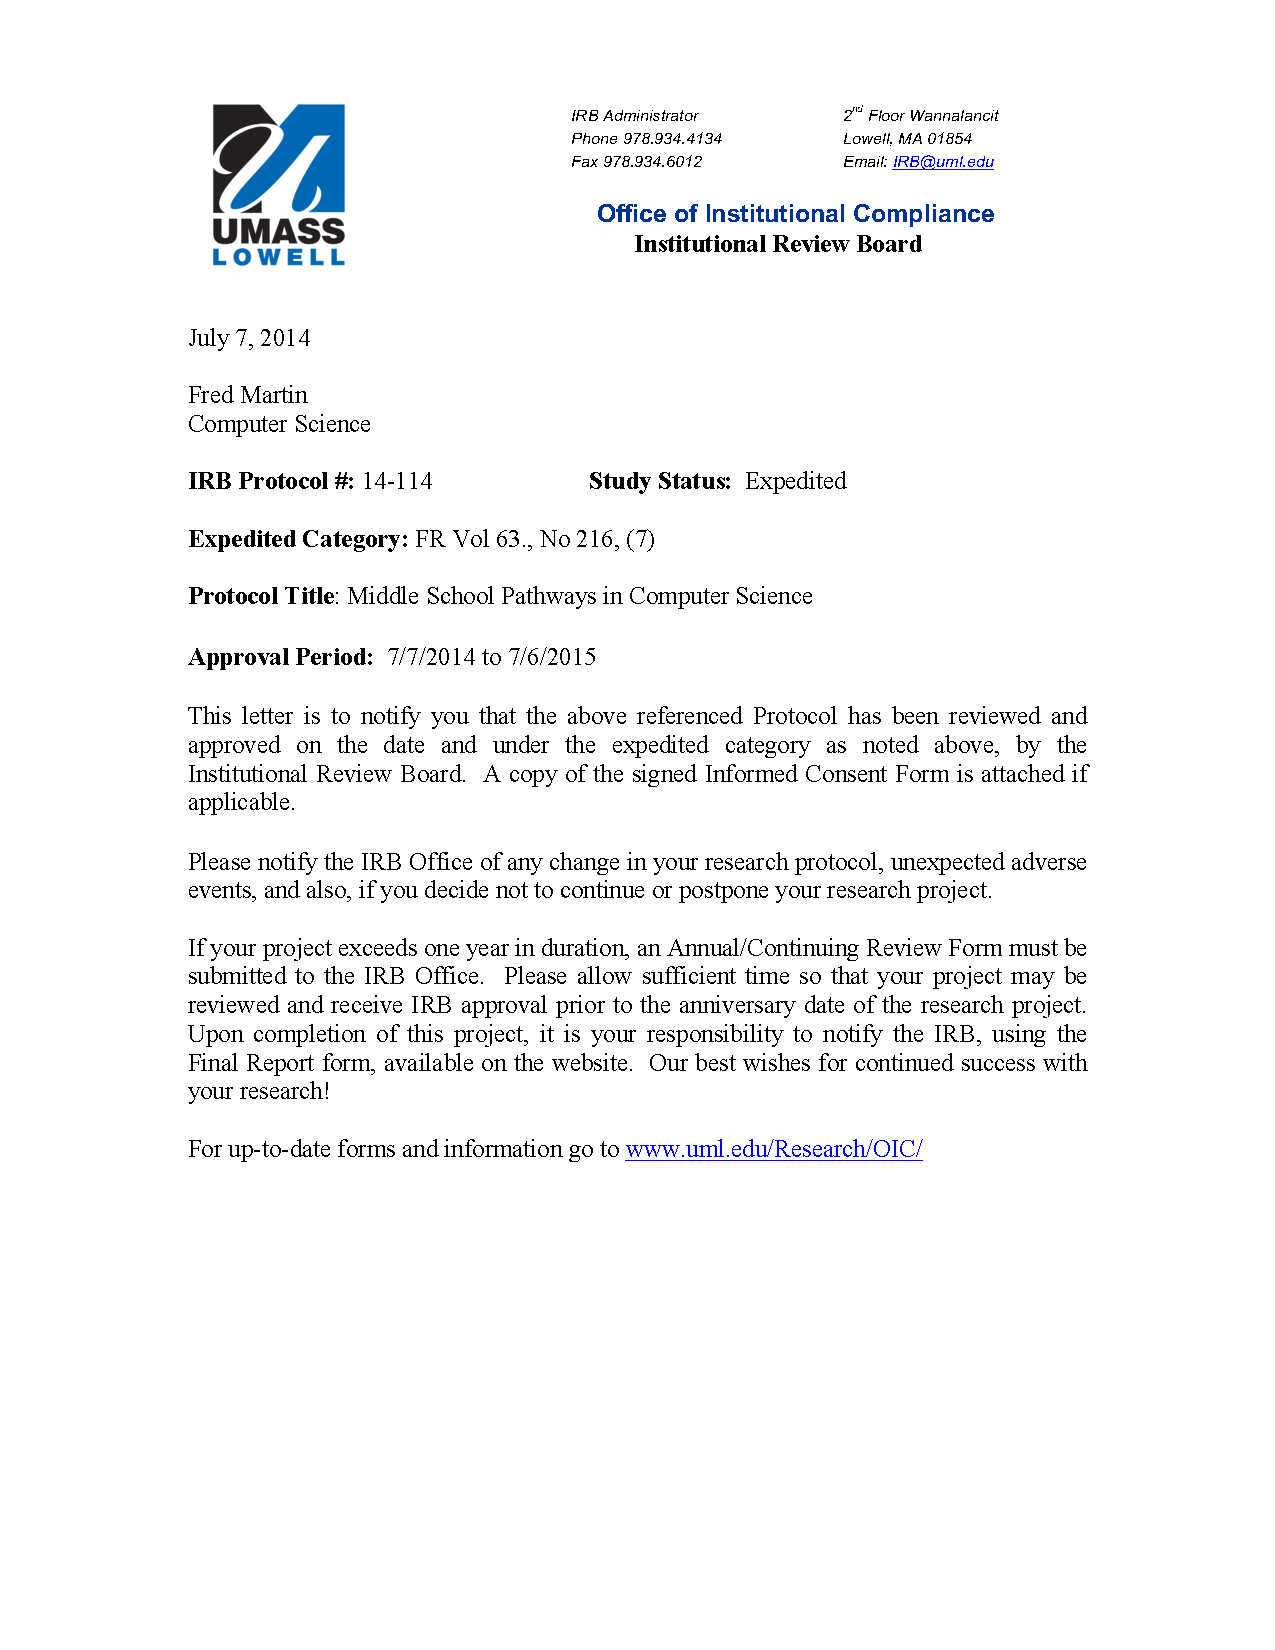
\includepdf[pages=-]{IRB/14-144-apv.pdf}

\section{The Debugging Activity and De-Identification Protocol}
This amendment added the author, Mark Sherman, and fellow researcher Lijun Ni to the project. This amendment also specified the Debugging Activity, and its protocol for classroom use. This amendment included the data de-identification protocol, which was discussed in Section \ref{sec:deident}.

The following pages contain the Debugging Game protocol description, including the de-identification protocol, a copy of the amendment application, and the approval letter.

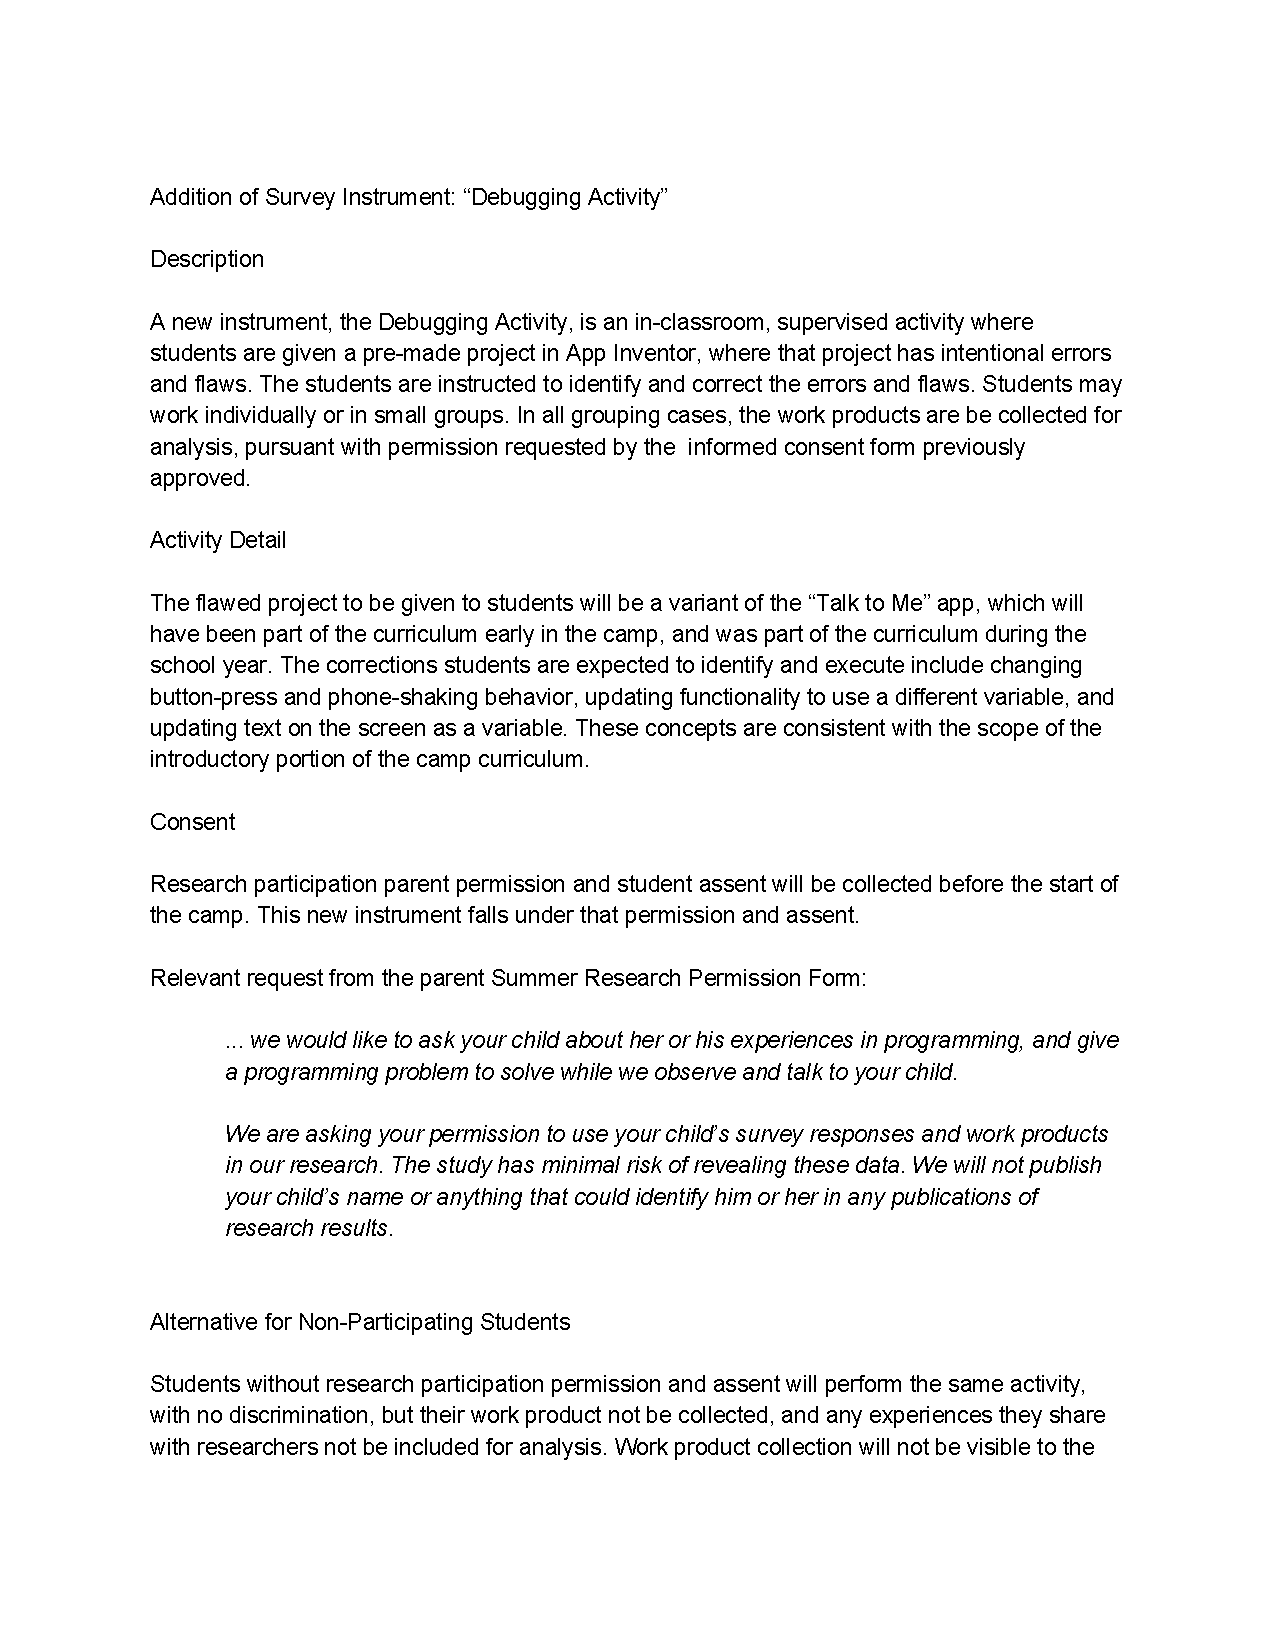
\includepdf[pages=-, frame, scale=.8]{IRB/AM2-DebuggingActivity2015.pdf}
%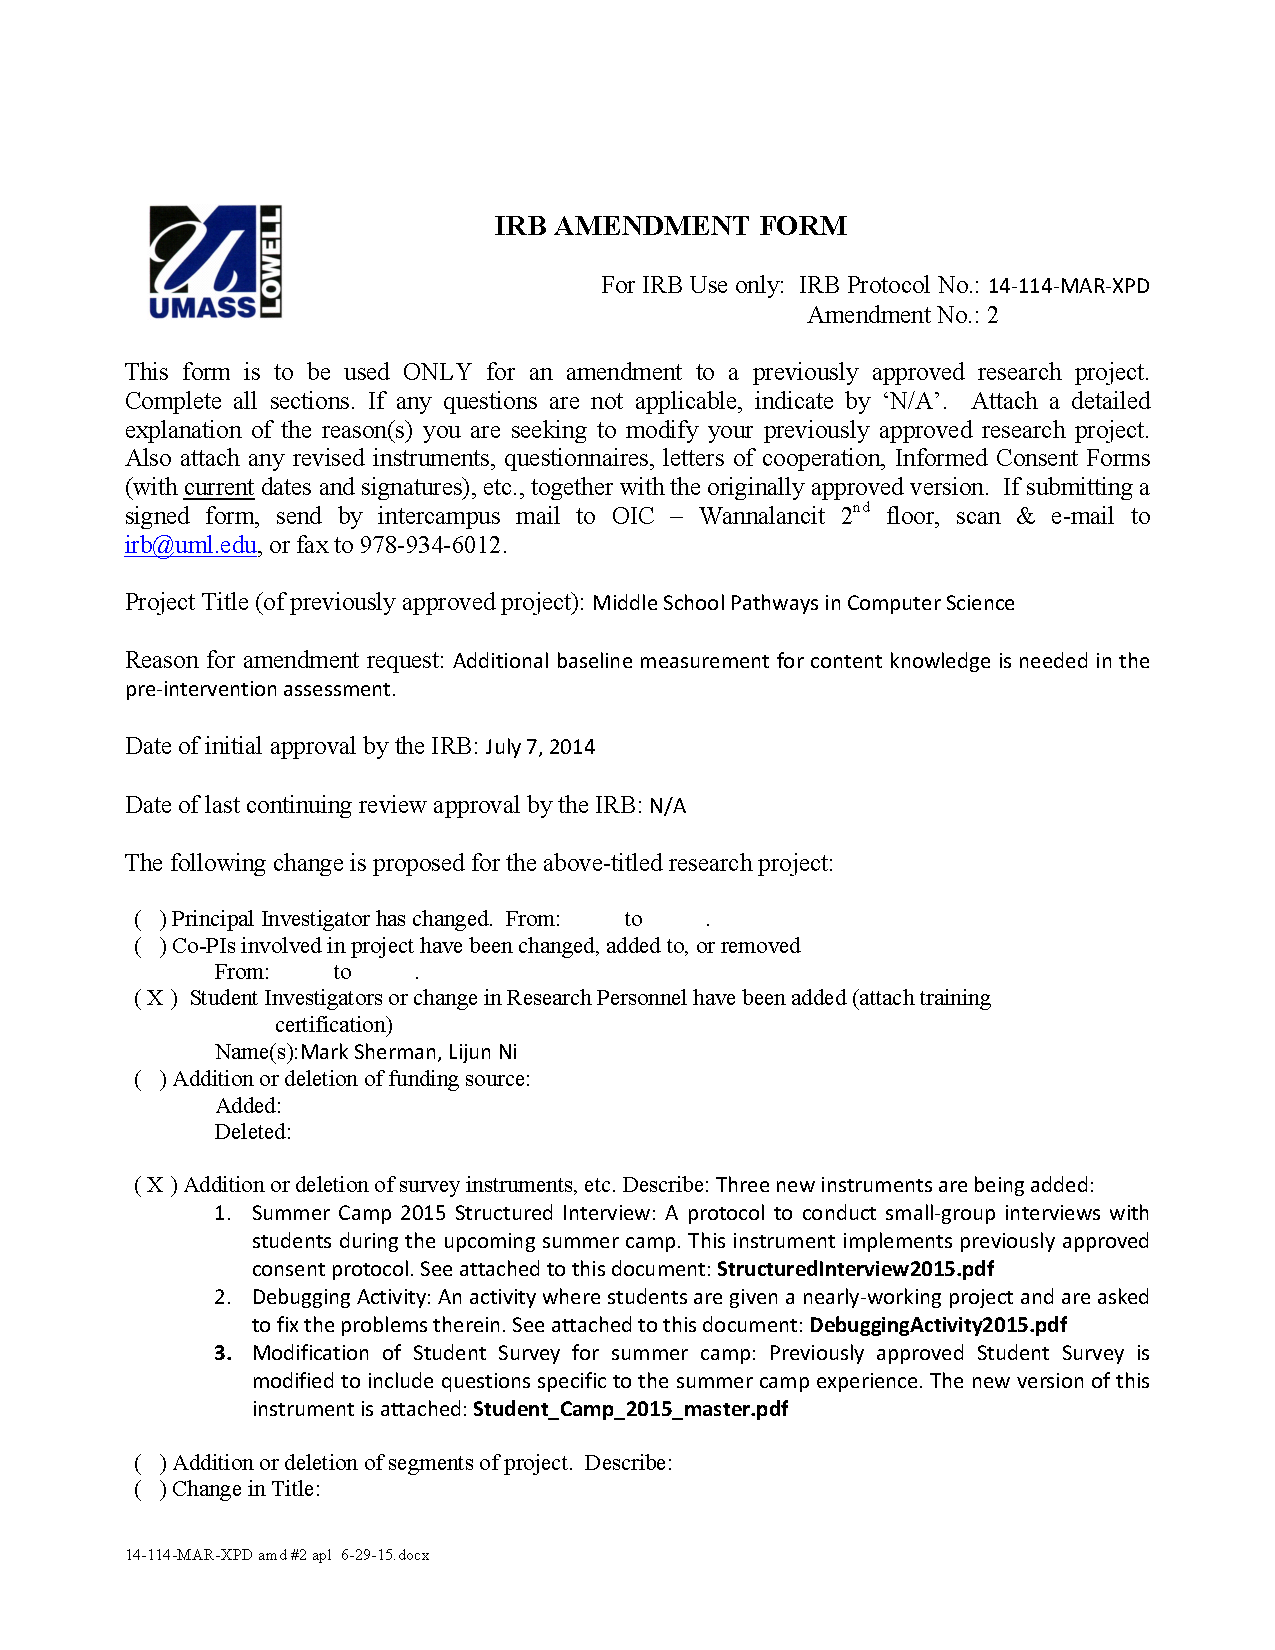
\includepdf[pages=-]{IRB/AM2-application.pdf}
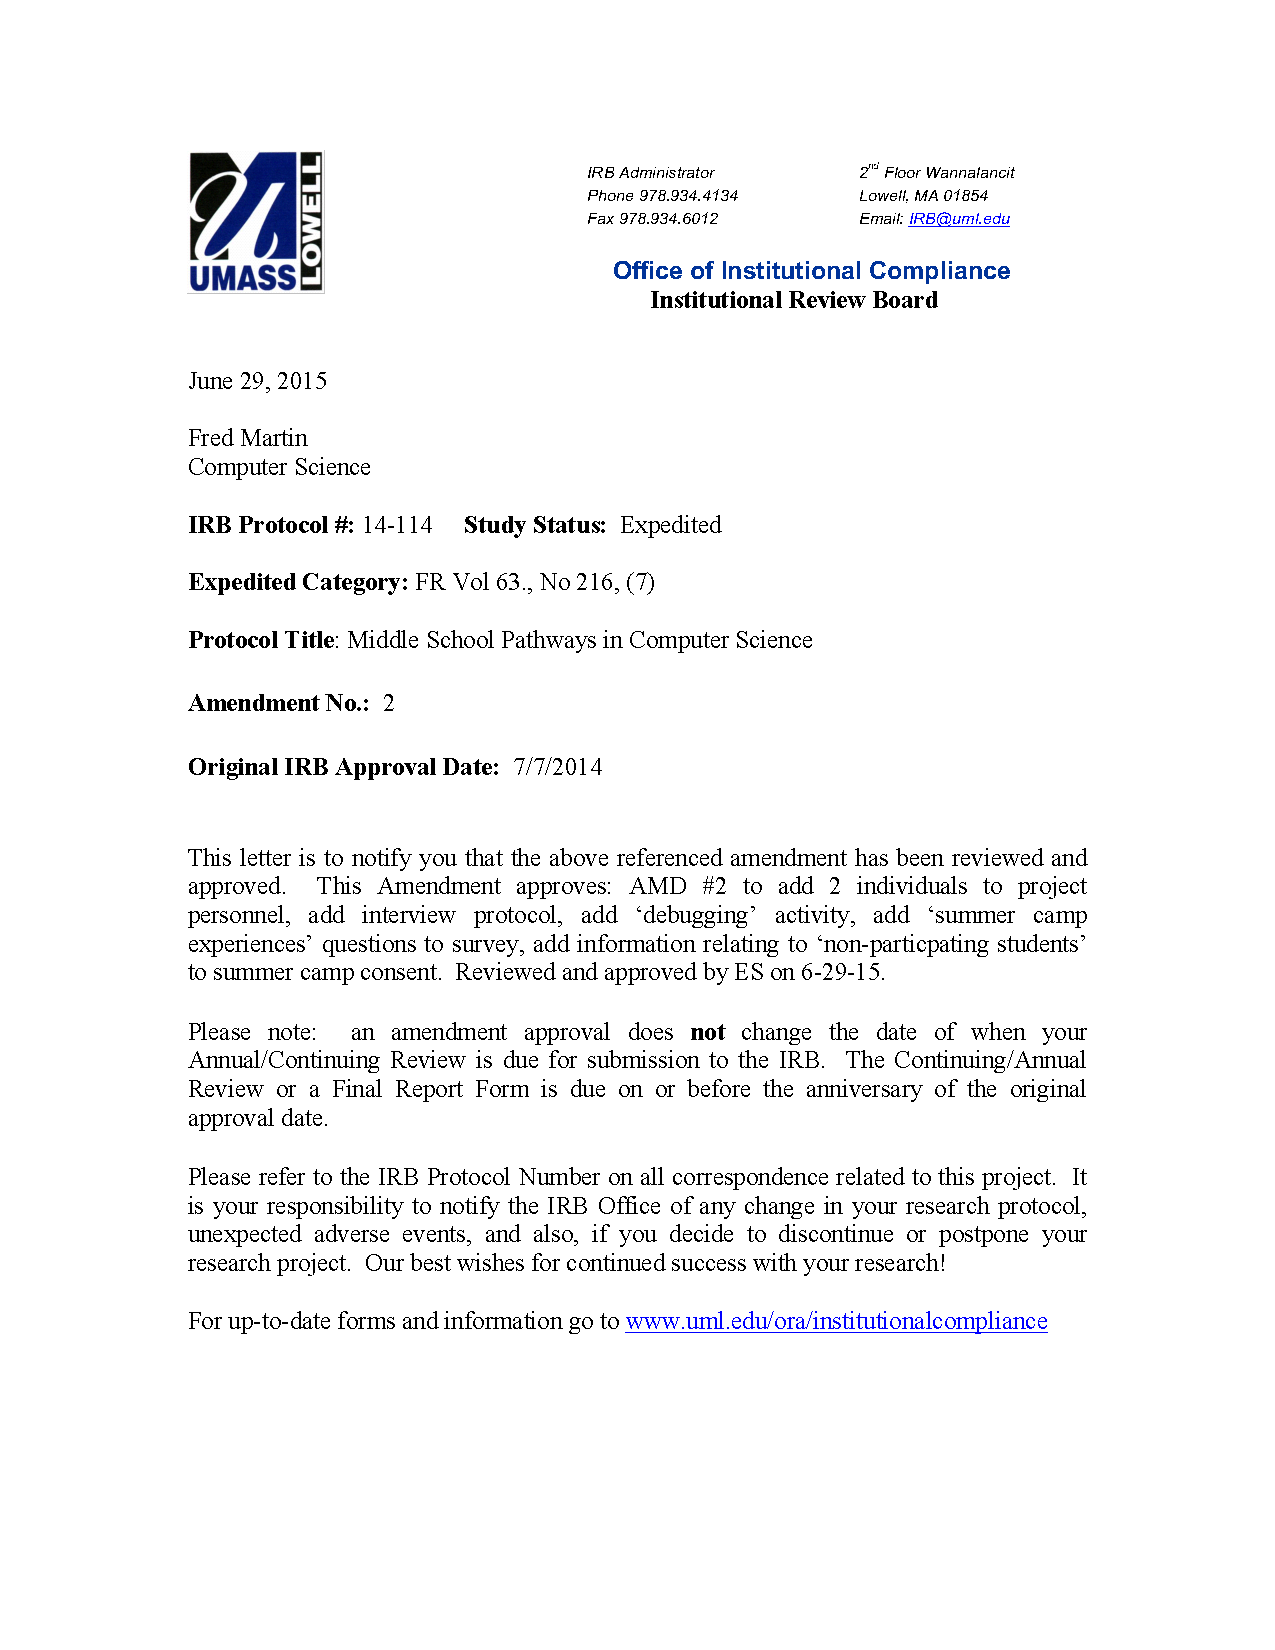
\includepdf[pages=-, frame, scale=.8]{IRB/AM2-approve.pdf}
\label{IRB:deident}


% \section{Annual/Continuing Review 2015}
% This application updated the IRB on the activities of the first year of the grant project, and declared intent for ongoing participant recruitment and data analysis until August 31, 2017. The following pages contain a copy of the review application and approval letter. The letter also mentions Amendment 3, which was approved at the same time, but is not relevant to the research in this document.

% 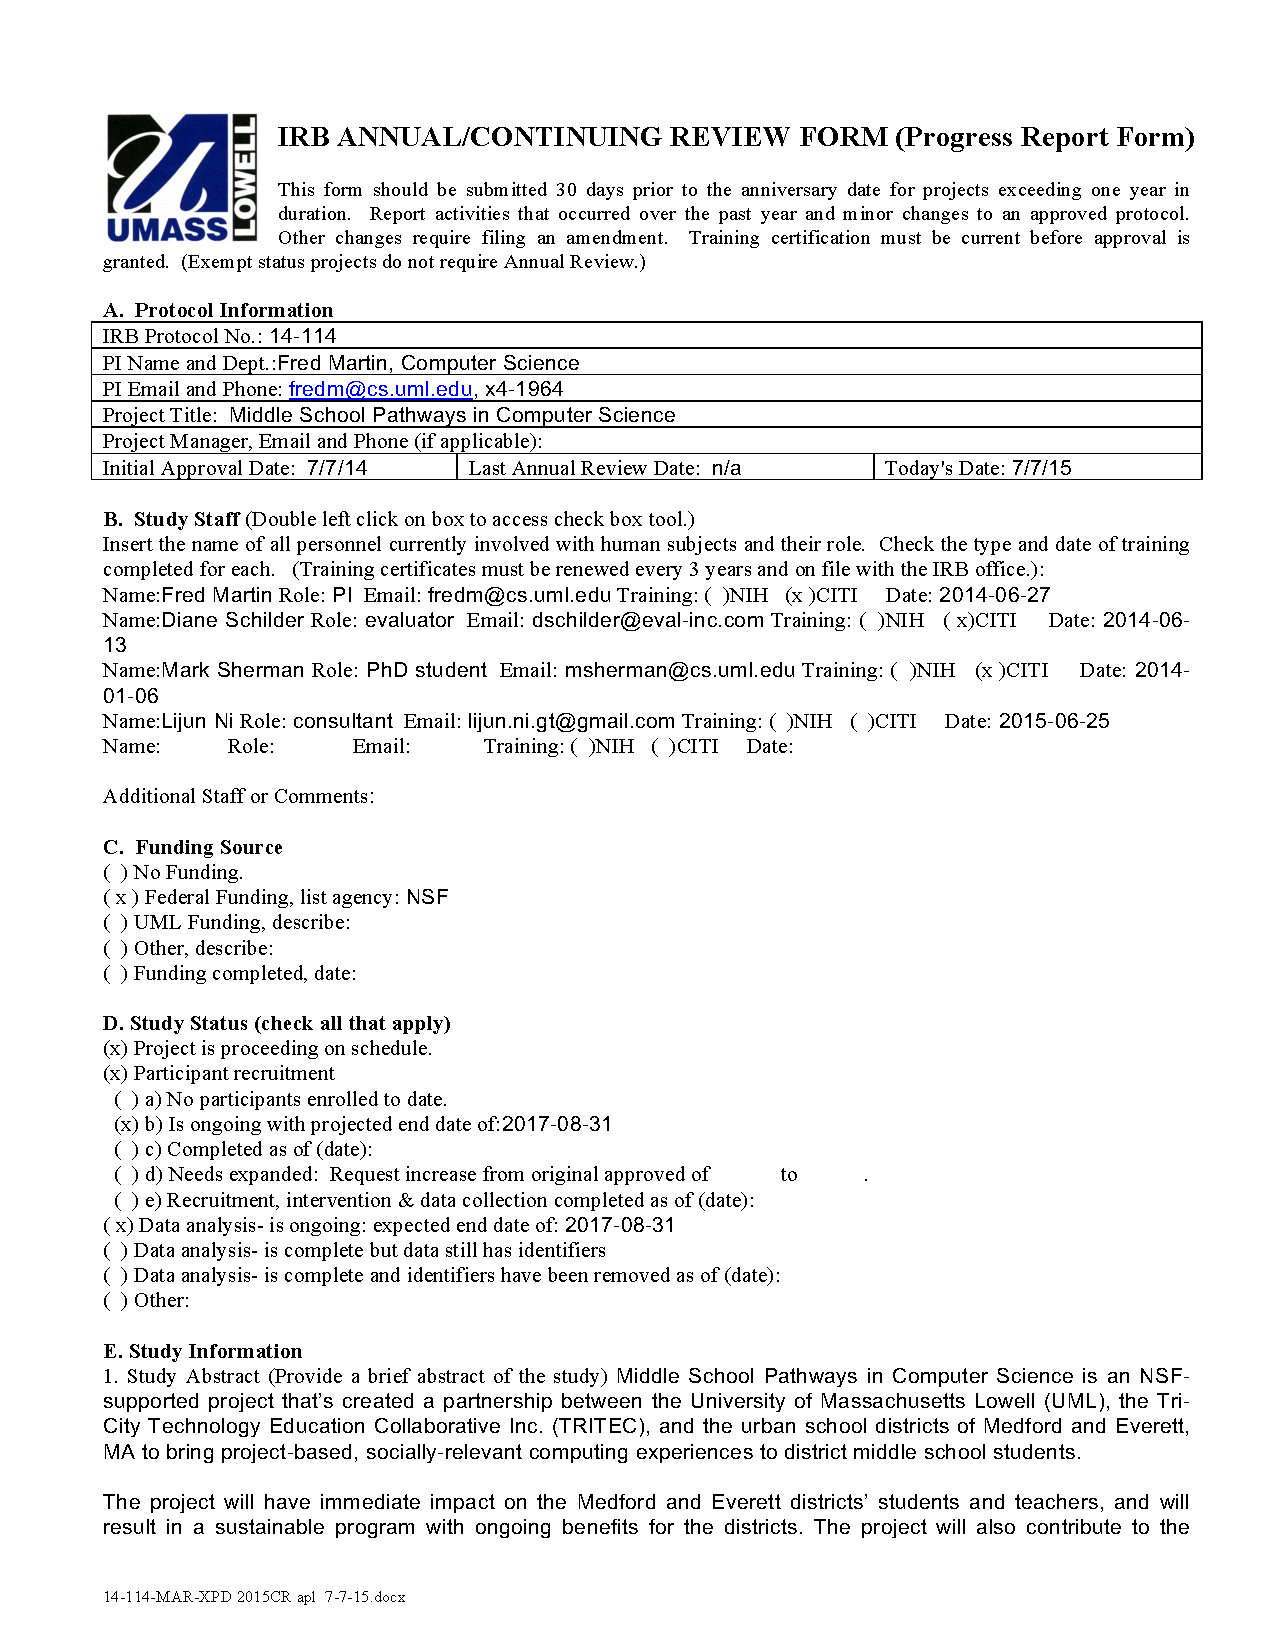
\includepdf[pages=-]{IRB/Year1-review-apl.pdf}
% 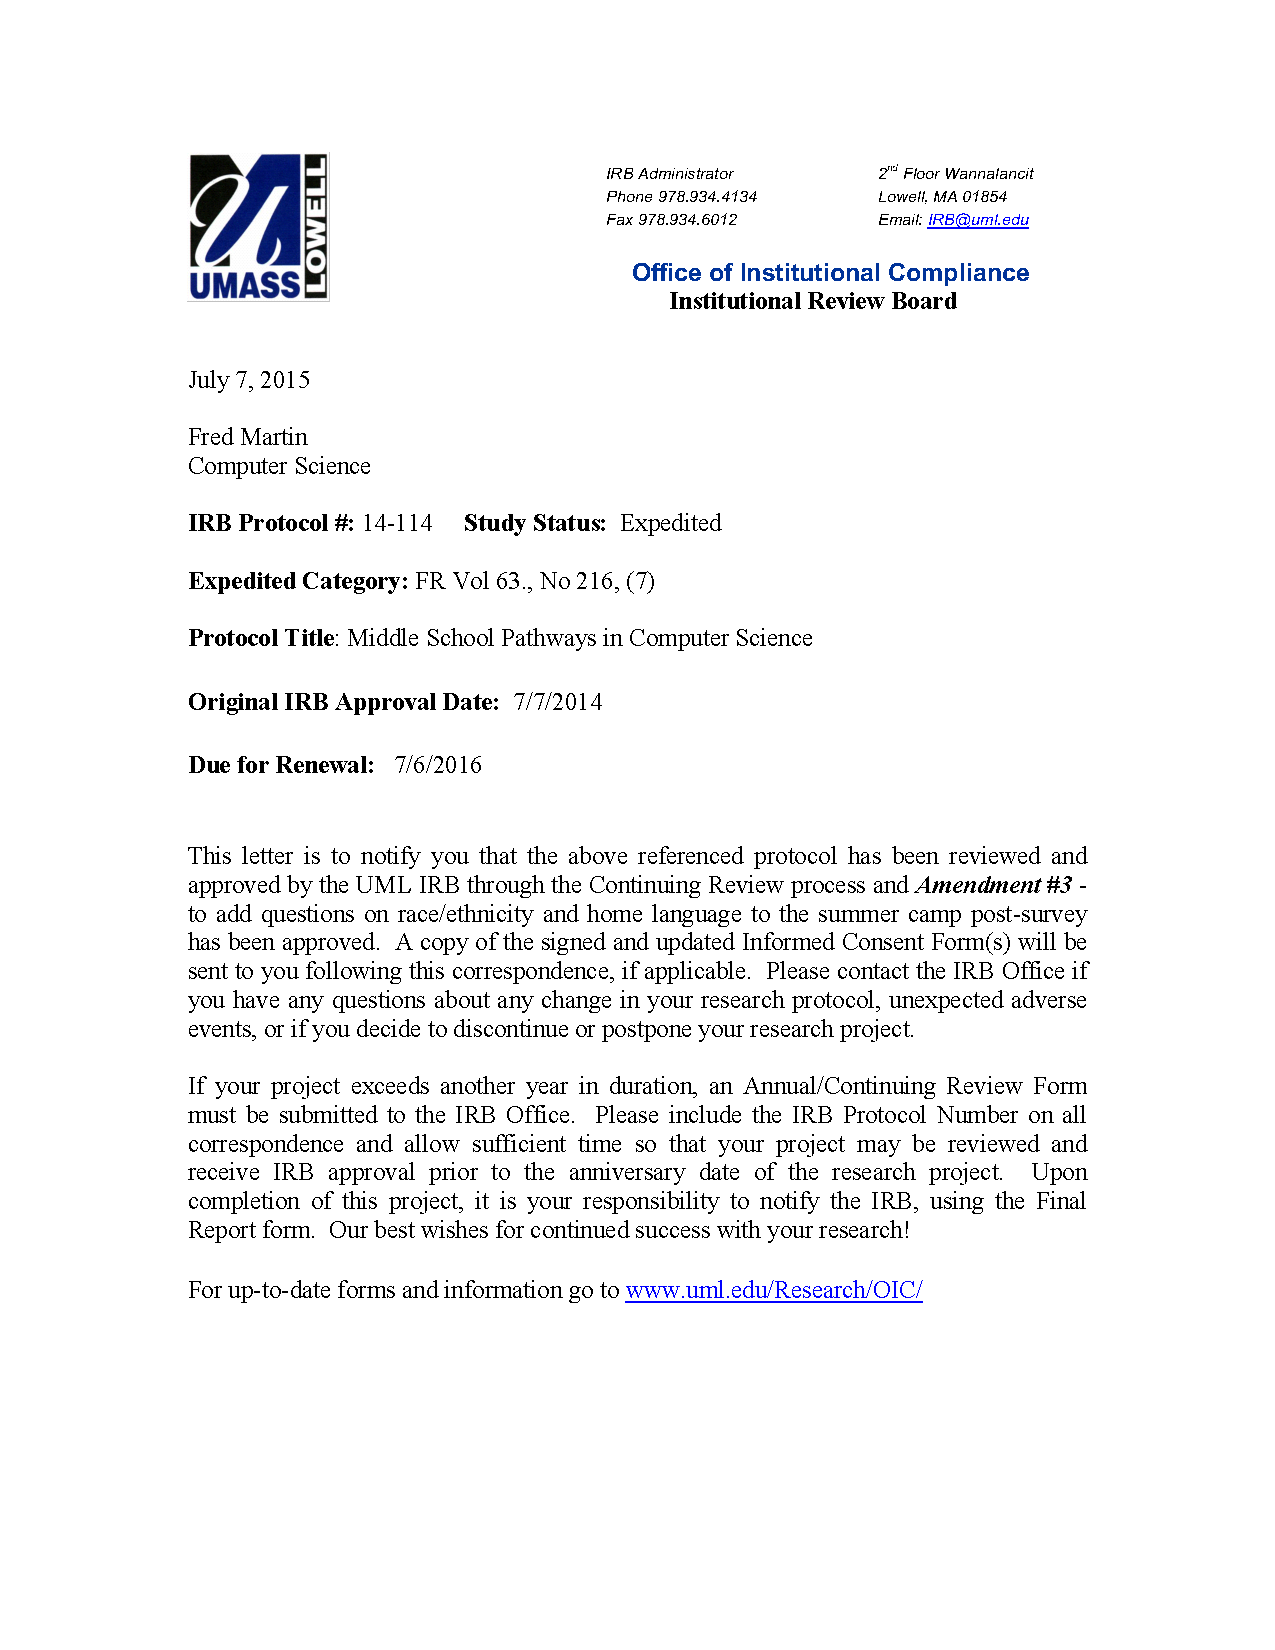
\includepdf[pages=-]{IRB/Year1-review-apv.pdf}

\section{Informed Consent, In-School}
\label{sec:icf:school}
The participants in this study were children, so an informed consent form was created for their parents, and a student assent form was provided to the children. The following pages are copies of those consent and assent forms as they were presented to the in-school cohort.
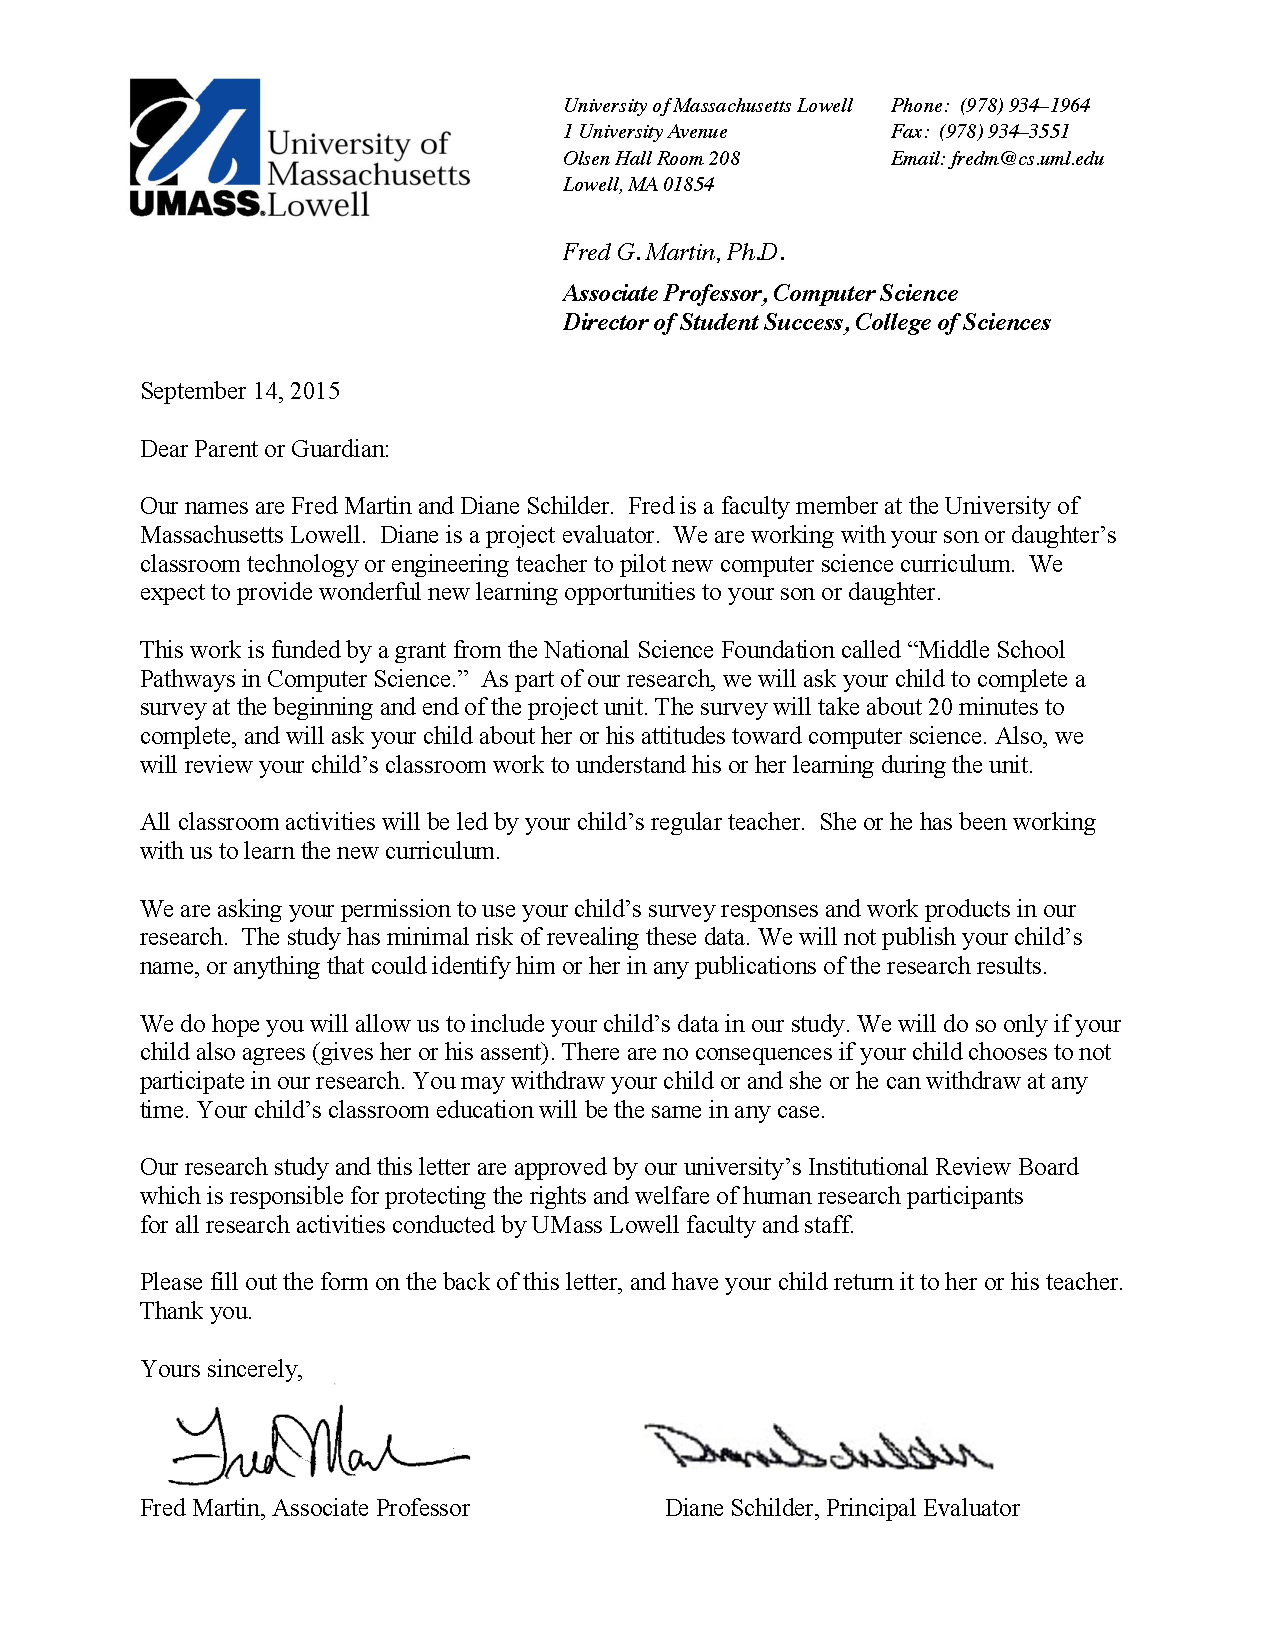
\includepdf[pages=-, frame, scale=.8]{IRB/icf-parent-in-school-rev3-9-14-15.pdf}
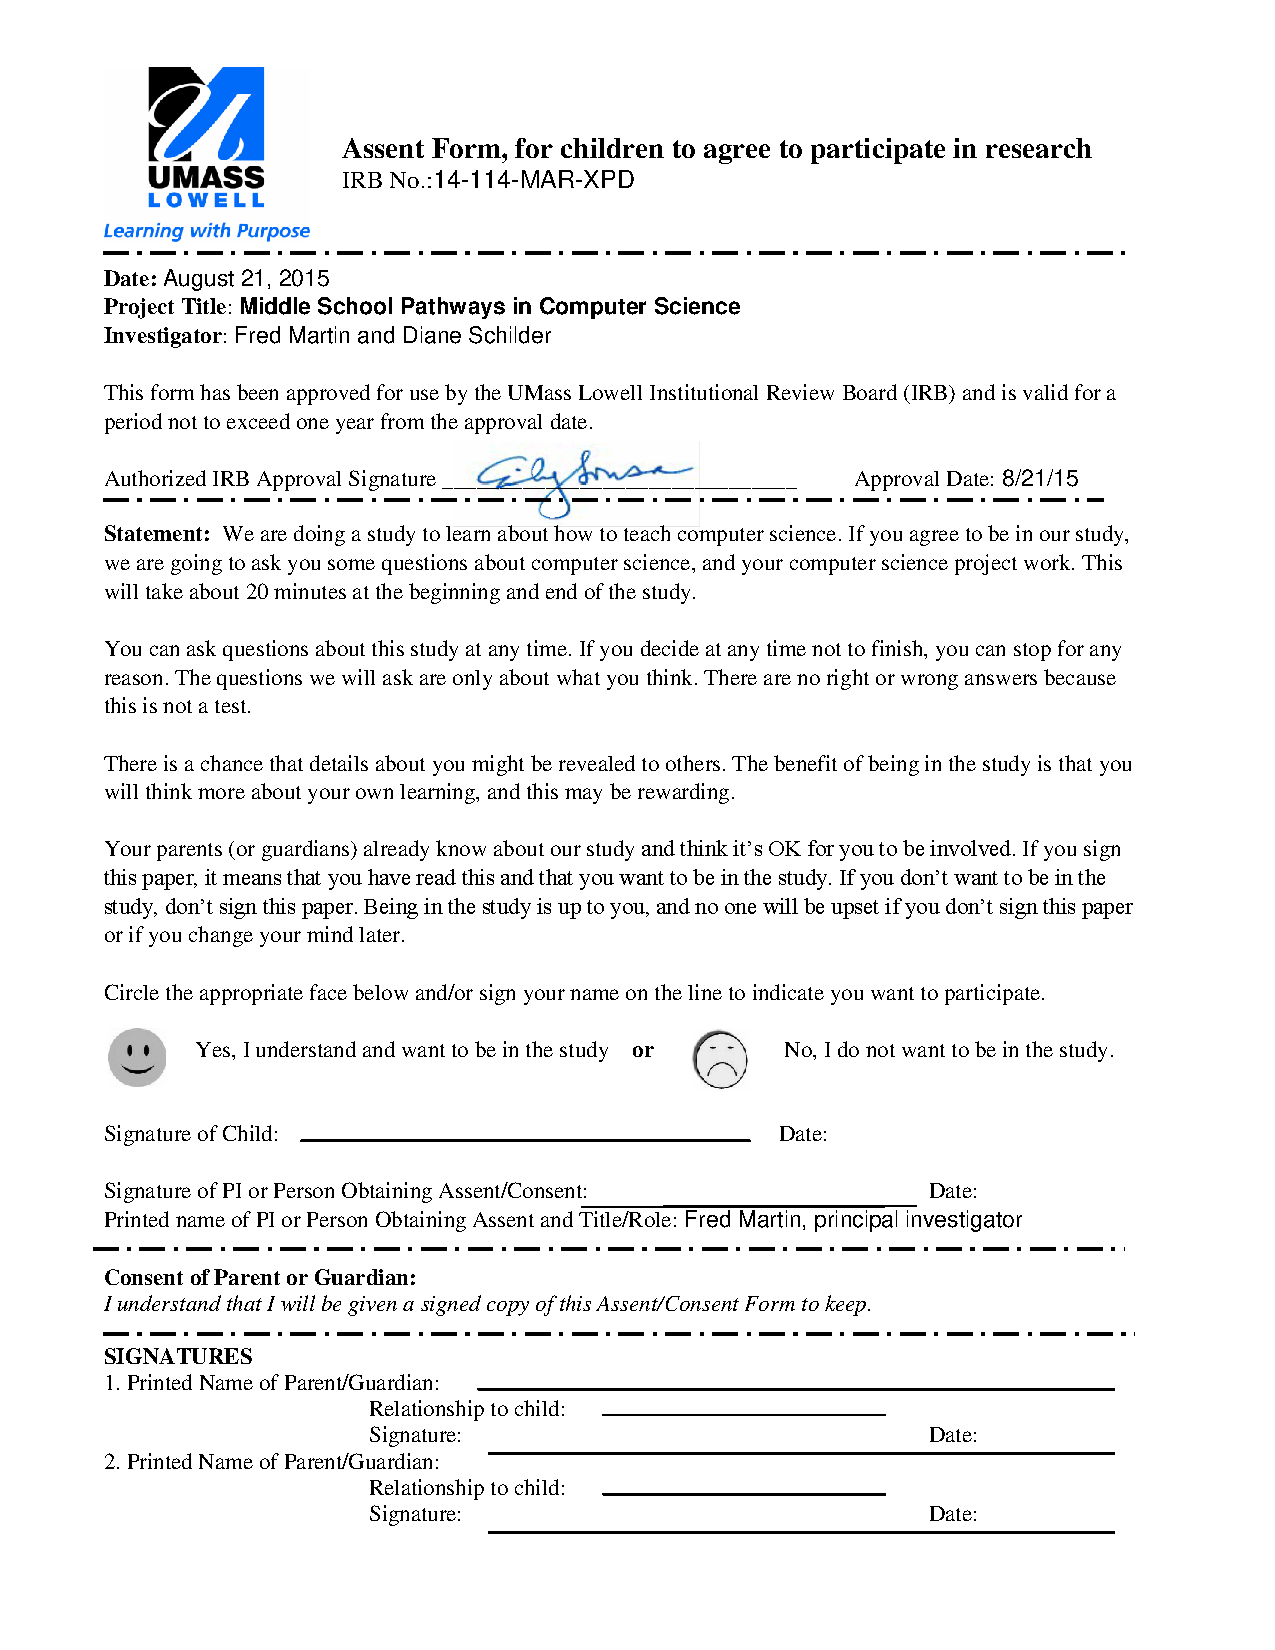
\includepdf[pages=-, frame, scale=.8]{IRB/icf-assent-8-21-15.pdf}


\section{Informed Consent, Summer Camp}
\label{sec:icf:camp}
The participants in this study were children, so an informed consent form was created for their parents, and a student assent form was provided to the children. The student assent form was unchanged from the In-School cohort (Appendix \ref{sec:icf:school}). The parental consent form was updated. The following pages are copies of the updated summer camp parental consent and the corresponding IRB approval letter.

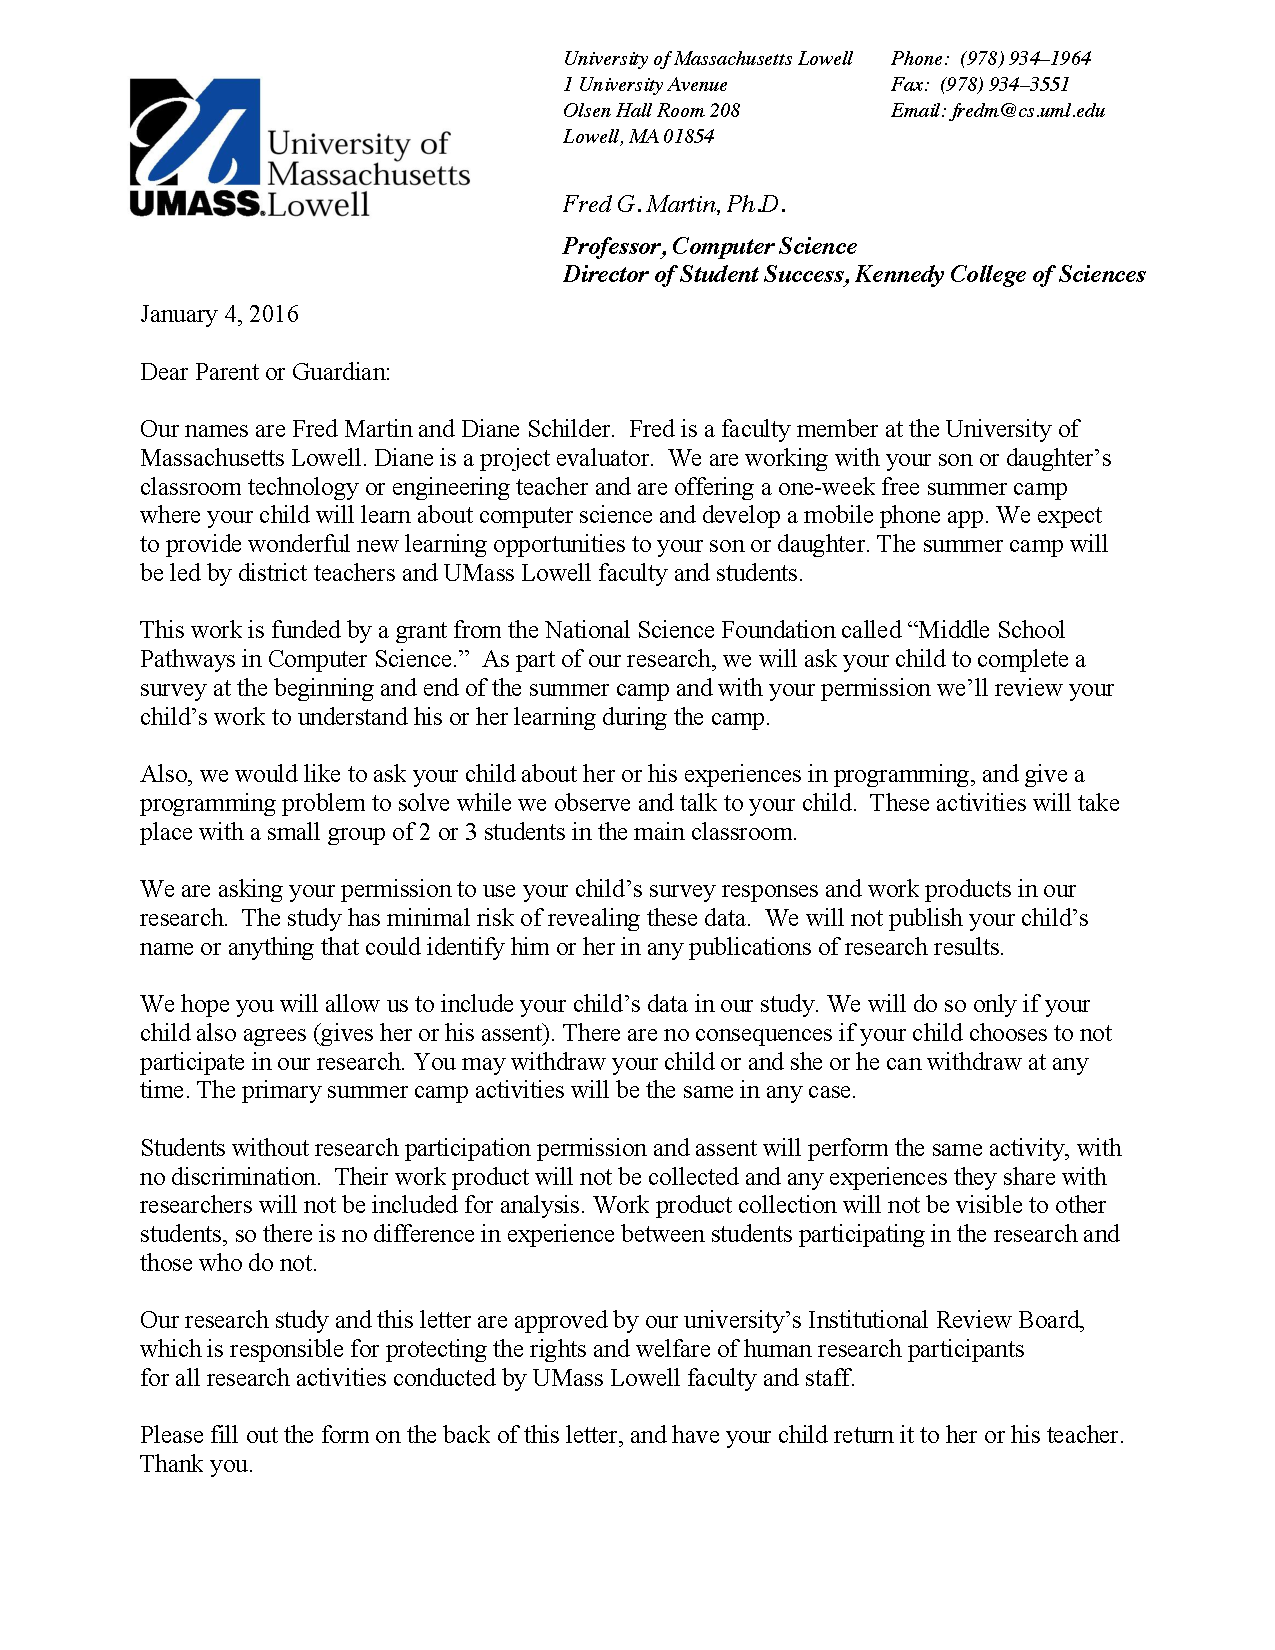
\includepdf[pages=-, frame, scale=.8]{IRB/icf-summer-camp-parent-consent-2016.pdf}
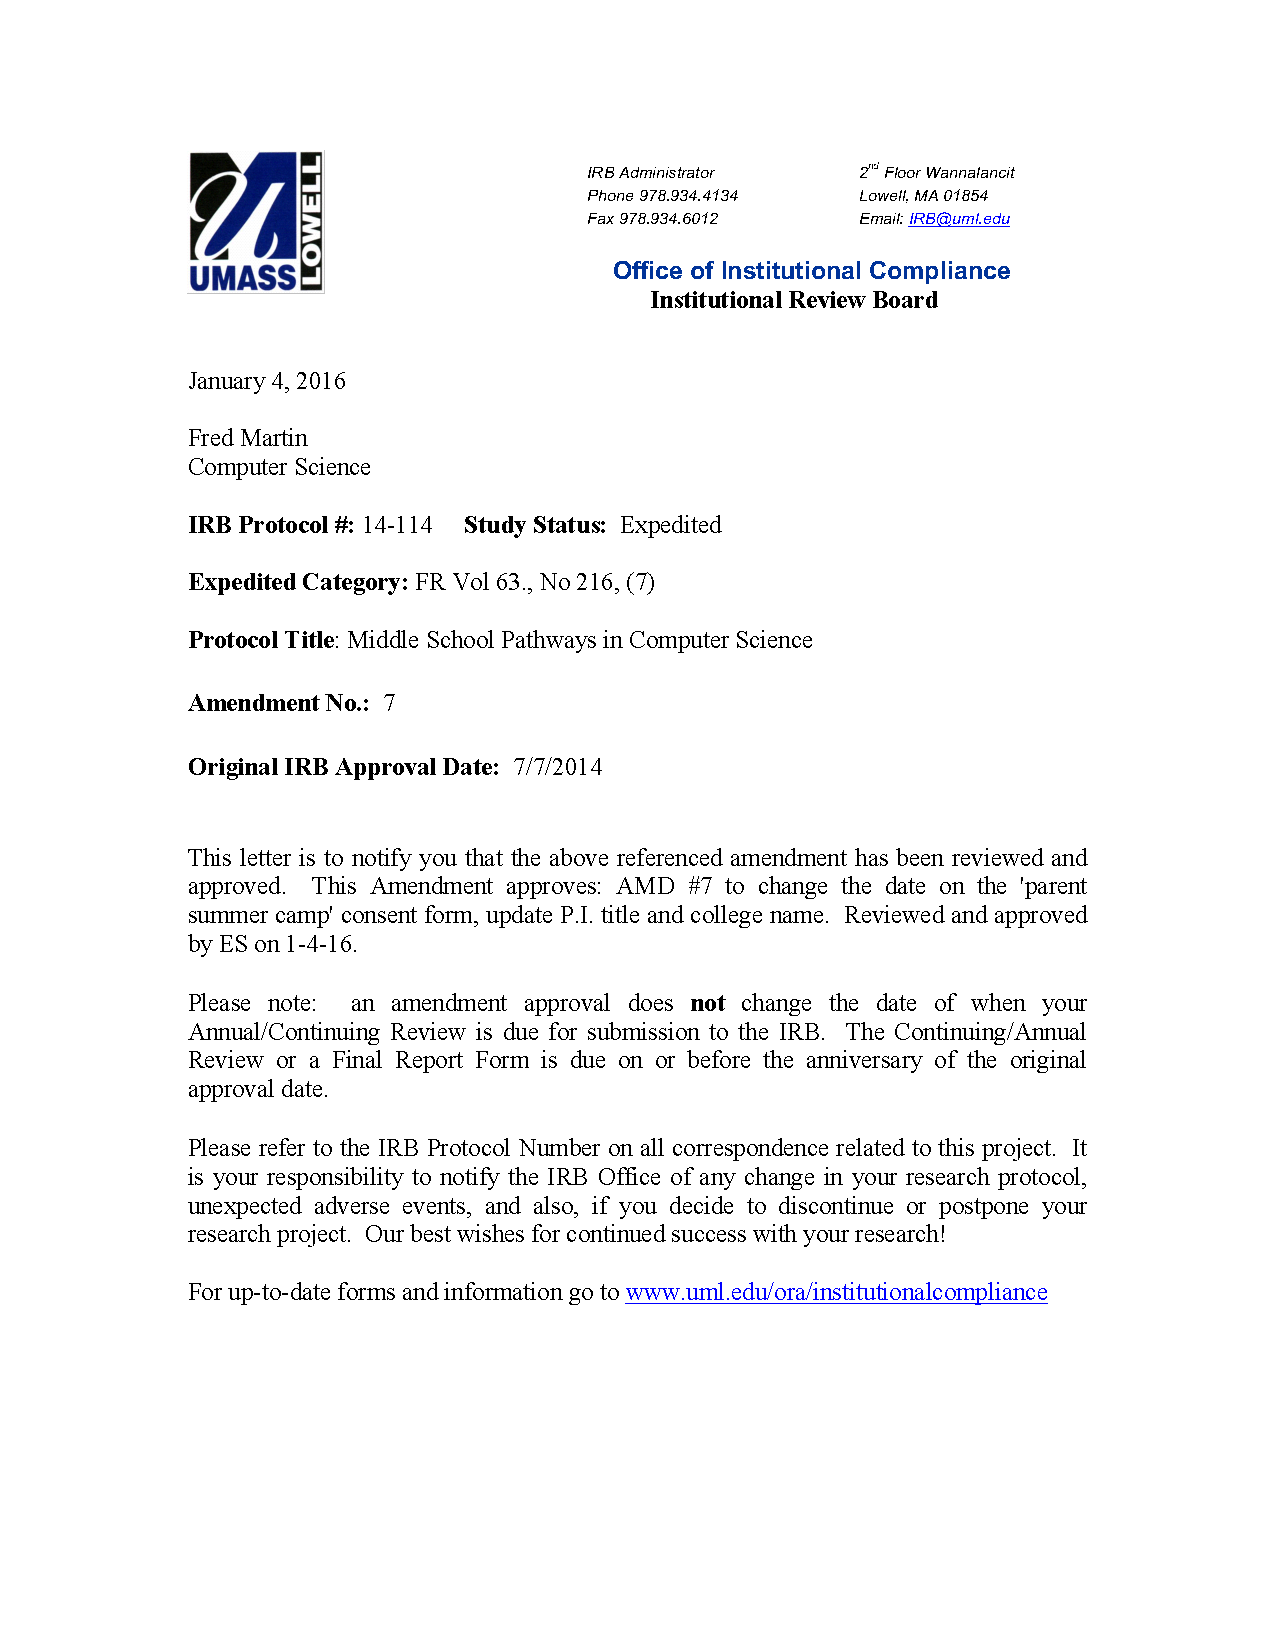
\includepdf[pages=-, frame, scale=.8]{IRB/icf-summer-camp-parent-consent-2016-approval.pdf}


% \section{Student Activities for Summer Camp Research}
% Amendment 10 added protocols for the Debugging Activity and Temperature Activity, both of which were used for data collection in this research. The protocol documents follow in Sections \ref{sec:IRB:debugging} and \ref{sec:IRB:temperature}, respectively. The following pages are copies of the IRB amendment form, and the approval letter affirming that these instruments operate under previously approved informed consent mechanisms. 

% 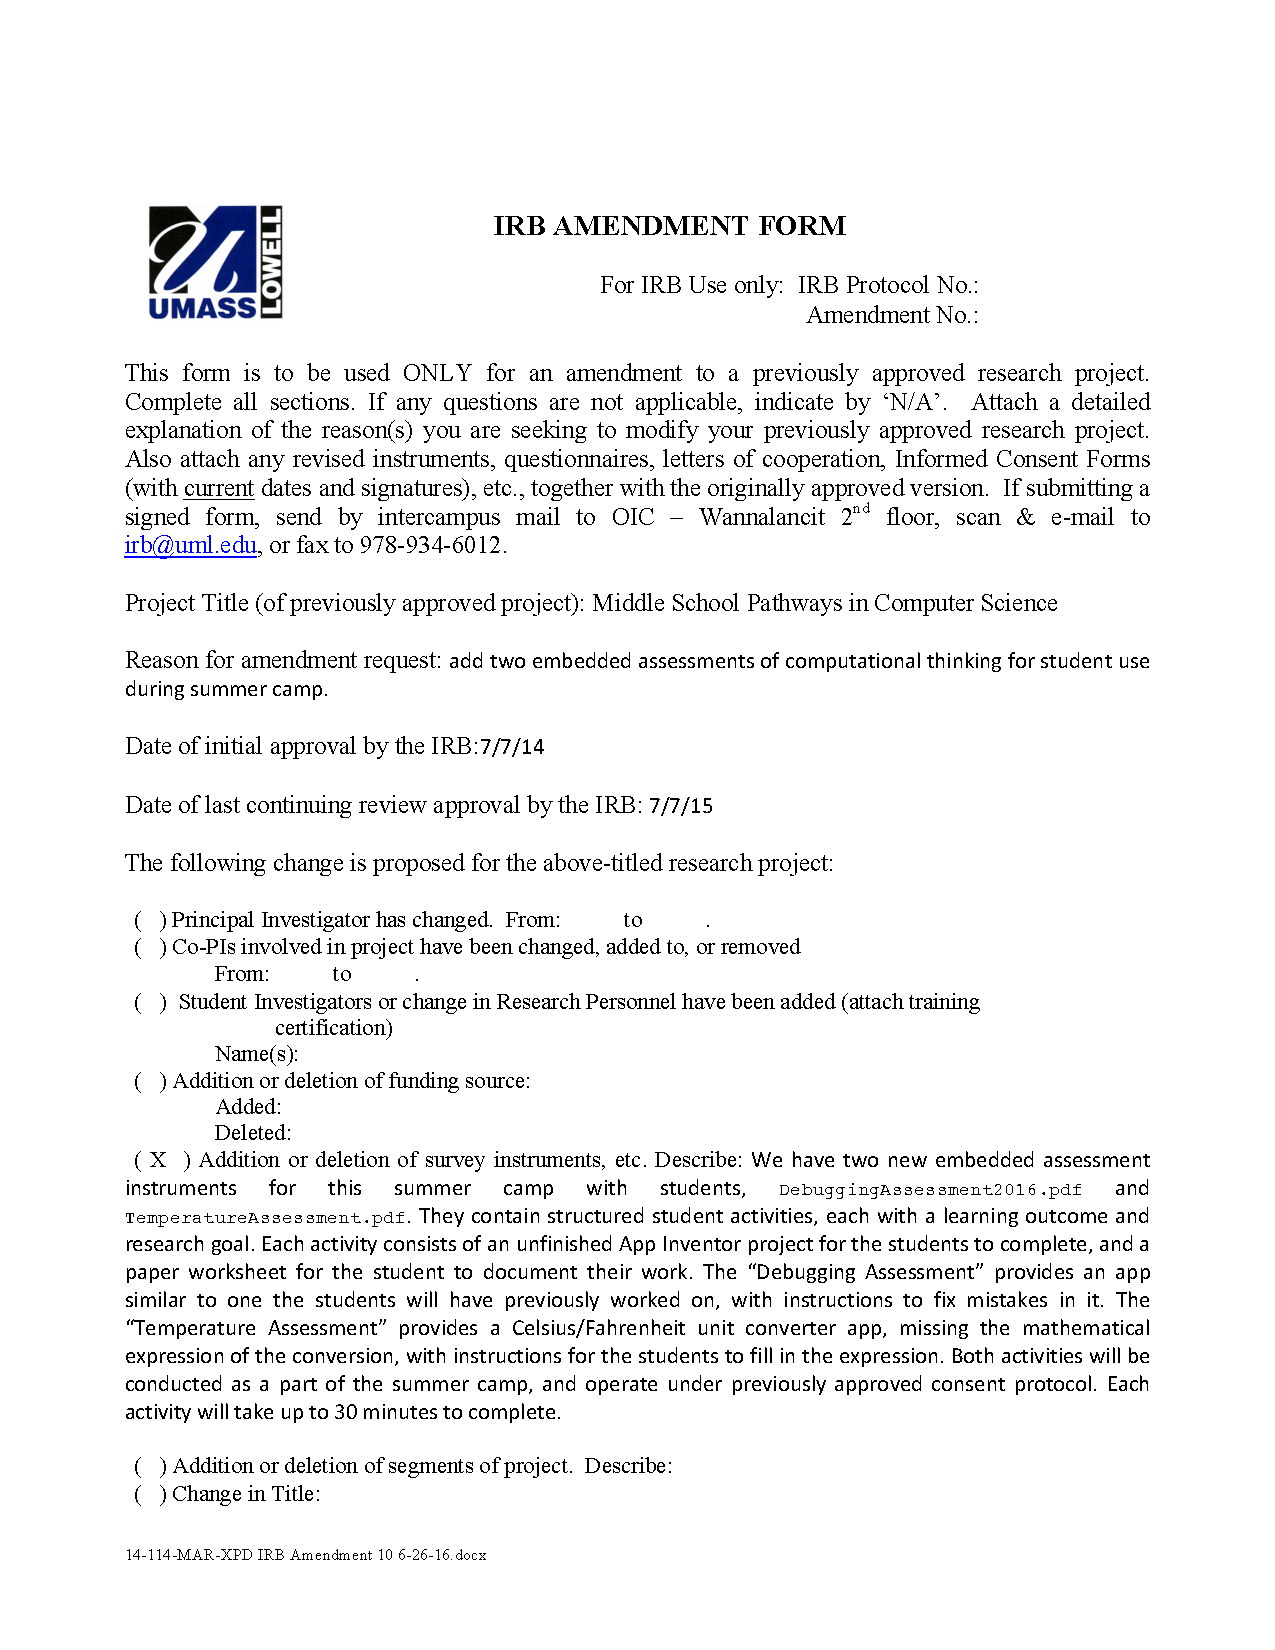
\includepdf[pages=-]{IRB/AM10-application.pdf}
% 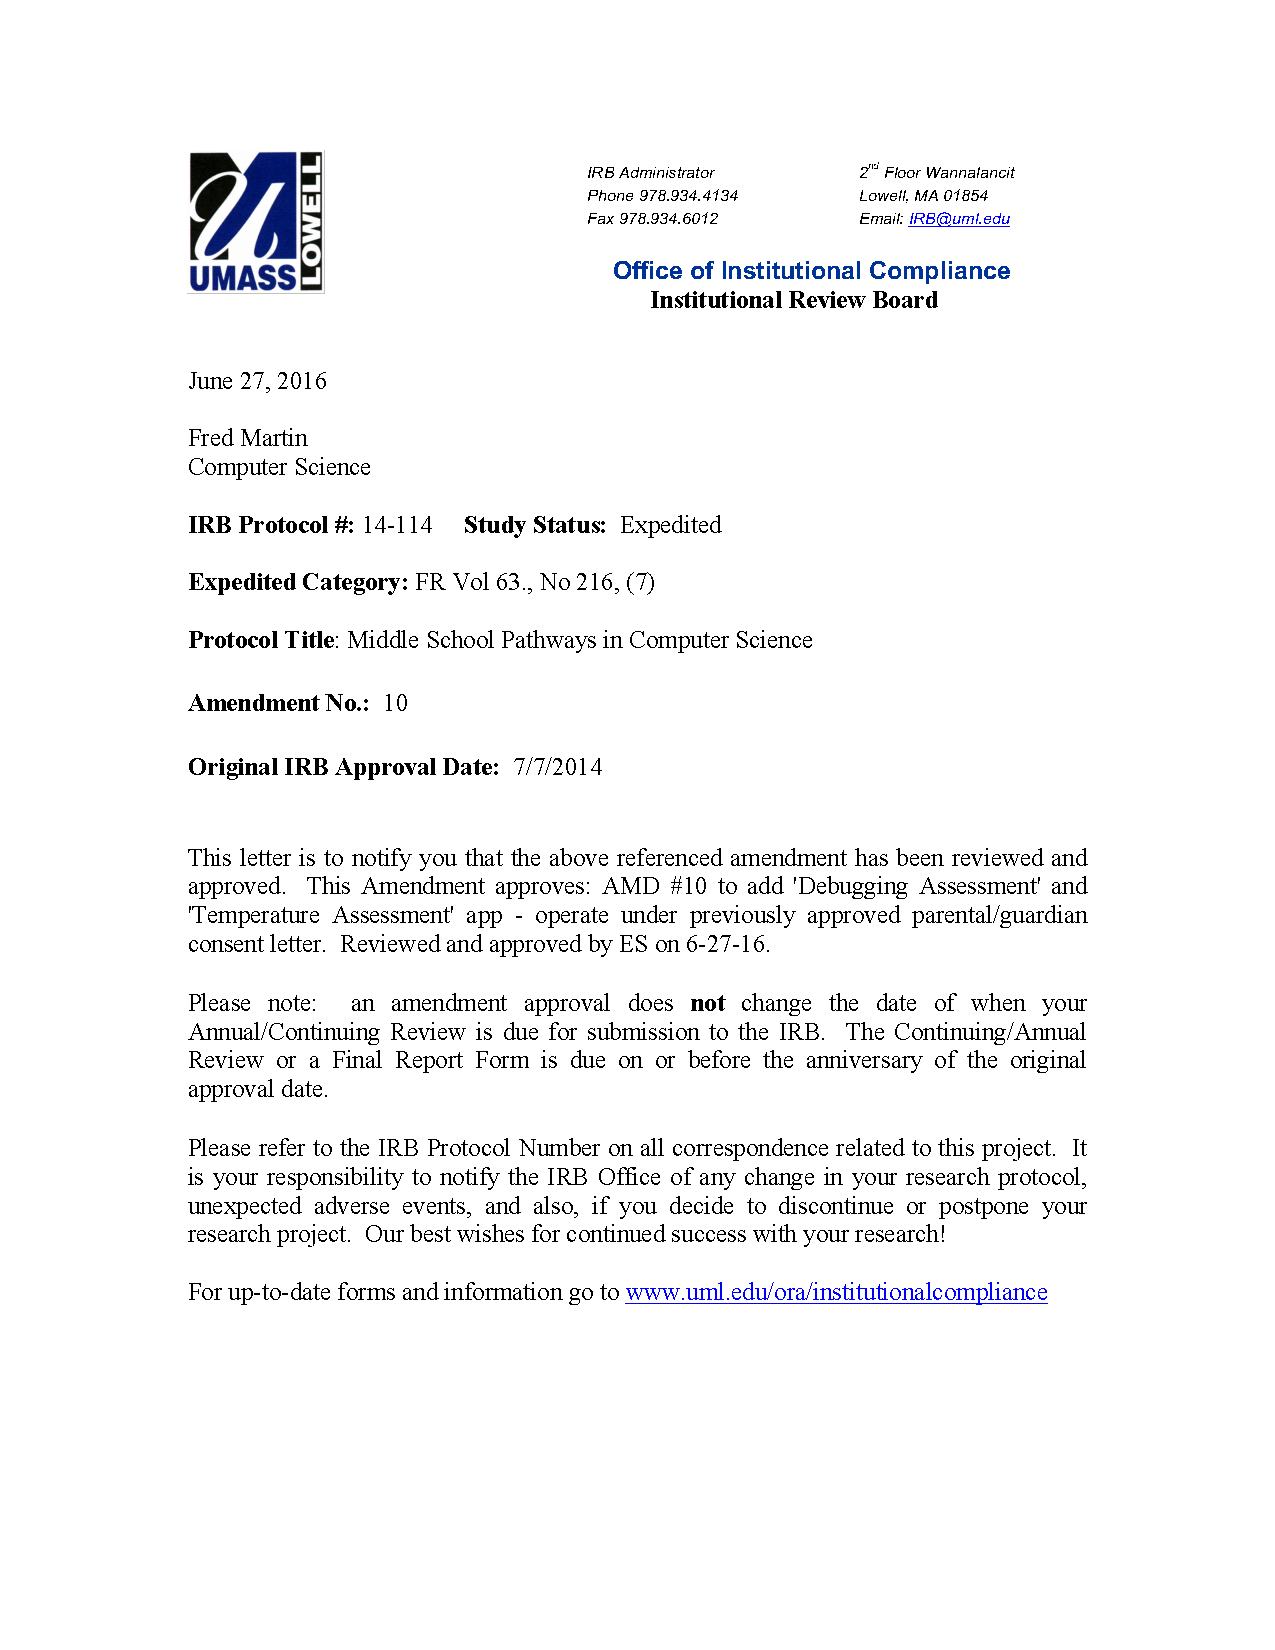
\includepdf[pages=-]{IRB/AM10-apv.pdf}

%%%%%%%%%%%%%%%%%%%%%%%%%%%%%%%%%%%%%%%%%%%%%%%%%%%%%%%%%%%%%%%%%%%%%%%%%%%%%%%%
%%%%%%%%%%%%%%%%%%%%%%%%%%%%%%%%%%%%%%%%%%%%%%%%%%%%%%%%%%%%%%%%%%%%%%%%%%%%%%%%

\chapter{Code Availability}

\noindent The App Inventor project, supported by the MIT Center for Mobile Learning, can be found here:

\noindent \url{https://github.com/mit-cml/appinventor-sources}

\noindent The modified version of App Inventor used in this project can be found in the author's github account:

\noindent \url{https://github.com/marksherman/appinventor-sources/tree/snapshot-service}

\noindent The long-term home for the features from this project is within the github home of the Engaging Computing Lab at UMass Lowell. That code can be found here:

\noindent \url{https://github.com/engaging-computing/appinventor-sources}

\noindent The source of this document is available from the author here:

\noindent \url{https://github.com/marksherman/umlthesis/tree/markphd}

\noindent The template used to write this document is available from the Engaging Computing lab at UMass Lowell:

\noindent \url{https://github.com/engaging-computing/umlthesis}

\noindent Especially relevant excerpts from the source code are listed in Appendix \ref{appendix:listings}.


